\section{FIR Filtering and Convolution\buch{Chapter 4}}
\subsection{Block Processing Methods}
\subsubsection{Convolution\buchSeite{121}}

\begin{align}
& \text{duration of data record} && T_L=LT && \text{Signal Samples} && L=T_Lf_s \notag \\
& x(n) && n=0,1,\ldots,L-1 && \text{sampling Time} && T \notag
\end{align}

\begin{tabular}{|l|l|l|}
	\hline
	$y(n)$		& direct and LTI forms of convolution	& $y(n)=\sum\limits_m h(m)x(n-m)=\sum\limits_m x(m)h(n-m)$
	\\ \hline
	$y(n)$		& convolution table form				& $y(n)=\sum\limits_{\substack{i,j \\ i+j=n}} h(i)x(j)$
	\\ \hline
\end{tabular}

\begin{multicols}{2}
\subsubsection{Direct Form\buchSeite{123}}
\begin{tabular}{|l|l|}
	\hline
	$h$		& $h=[h_0,h_1, \ldots , h_M]$
	\\ \hline
	$L_h$	& $L_h = M + 1$
	\\ \hline
	$L_x$	& $L_x = L$
	\\ \hline
	$L_y$	& $L_y = L + M = L_x + L_h - 1$
	\\ \hline
	$y(n)$	& $y(n) = \sum\limits_{m=max(0,n-L+1)}^{min(n,M)} h(m)x(n-m)$
	\\ \hline 
\end{tabular}

\columnbreak

\subsubsection{Convolution Table\buchSeite{126}}

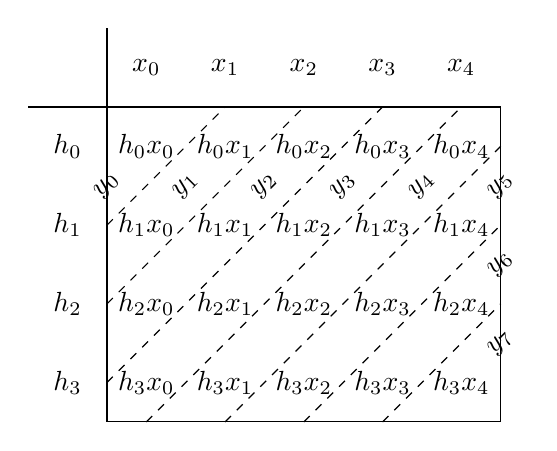
\begin{tikzpicture}
%lines
\draw (-0.5,3.5) -- (5.5, 3.5) -- (5.5,-0.5) -- (0.5,-0.5) -- (0.5,4.5);
\draw [dashed] (0.5,2) -- (2,3.5);
\draw [dashed] (0.5,1) -- (3,3.5);
\draw [dashed] (0.5,0) -- (4,3.5);
\draw [dashed] (1,-0.5) -- (5,3.5);
\draw [dashed] (2,-0.5) -- (5.5,3);
\draw [dashed] (3,-0.5) -- (5.5,2);
\draw [dashed] (4,-0.5) -- (5.5,1);

%nodes
\foreach \h in {0,1,2,3} {
	\node at (0,3-\h) {$h_{\h}$};
};
\foreach \x in {0,1,2,3,4} {
	\node at (\x+1, 4) {$x_{\x}$};
	\foreach \h in {0,1,2,3} {
		\node at (\x+1, 3-\h) {$h_{\h}x_{\x}$};
	};
};
\foreach \n in {0,...,5} {
	\node [rotate=45] at (\n+0.5,2.5) {$y_{\n}$};
};
\node [rotate=45] at (5.5,1.5) {$y_6$};
\node [rotate=45] at (5.5,0.5) {$y_7$};

\end{tikzpicture}

$y=[y_0, y_1, y_2, y_3, y_4, y_5, y_6, y_7]$

\end{multicols}

\subsubsection{LTI Form\buchSeite{127}}
\begin{tabular}{c|c:c:c:c:c:c:c:c|}
	& $h_0$ & $h_1$ & $h_2$ & $h_3$ & 0 & 0 & 0 & 0 \\
	\hline
	$x_0$ & $x_0h_0$ & $x_0h_1$ & $x_0h_2$ & $x_0h_3$ & 0 & 0 & 0 & 0 \\
	$x_1$ & 0 & $x_1h_0$ & $x_1h_1$ & $x_1h_2$ & $x_1h_3$ & 0 & 0 & 0 \\
	$x_2$ & 0 & 0 & $x_2h_0$ & $x_2h_1$ & $x_2h_2$ & $x_2h_3$ & 0 & 0 \\
	$x_3$ & 0 & 0 & 0 & $x_3h_0$ & $x_3h_1$ & $x_3h_2$ & $x_3h_3$ & 0 \\
	$x_4$ & 0 & 0 & 0 & 0 & $x_4h_0$ & $x_4h_1$ & $x_4h_2$ & $x_4h_3$ \\
	\hline\hline
	$y_n$ & $y_0$ & $y_1$ & $y_2$ & $y_3$ & $y_4$ & $y_5$ & $y_6$ & $y_7$ \\
\end{tabular}
\begin{minipage}{6.5cm}
  \hspace{0.5cm} $y(n) = \sum\limits_{m=max(0,n-M)}^{min(n,L-1)} x(m)h(n-m)$
\end{minipage}


\subsubsection{Matrix Form\buchSeite{129}}
The convolutional equations can also be written in the linear matrix form:
\[
	y = H  x	\qquad \text{or} \qquad y = Xh
\]
where $H$ (Toeplitz Matrix) is built out of the filter's impulse response $h$ or the signal matrix $X$ is built 
out of the input signal. The filter matrix $H$, respectively the signal matrix $X$, must be rectangular with dimensions
\[
	\underbrace{L_y \times L_x = (L + M)\times L}_{\text{dimension of H}} \qquad \text{or} \qquad
	\underbrace{L_y \times L_h = (L + M)\times (M + 1)}_{\text{dimension of X}}
\]

Example:
\setArrayStretch{1}
\[
	y =
	\begin{bmatrix}
		y_0 \\
		y_1 \\
		y_2 \\
		y_3 \\
		y_4 \\
		y_5 \\
		y_6 \\
		y_7
	\end{bmatrix}
	= \begin{bmatrix}
		h_0	& 0		& 0		& 0		& 0 \\
		h_1	& h_0	& 0 	& 0 	& 0 \\
		h_2	& h_1	& h_0	& 0		& 0 \\
		h_3 & h_2	& h_1	& h_0	& 0 \\
		0	& h_3	& h_2	& h_1	& h_0 \\
		0	& 0		& h_3	& h_2	& h_1 \\
		0	& 0		& 0		& h_3	& h_2 \\
		0	& 0		& 0		& 0		& h_3	 
	  \end{bmatrix}
	  \begin{bmatrix}
	  	x_0 \\
	  	x_1 \\
	  	x_2 \\
	  	x_3 \\
	  	x_4
	  \end{bmatrix}
	= Hx
\]
\resetArrayStretch


\subsubsection{Flip-and-Slide Form\buchSeite{131}}
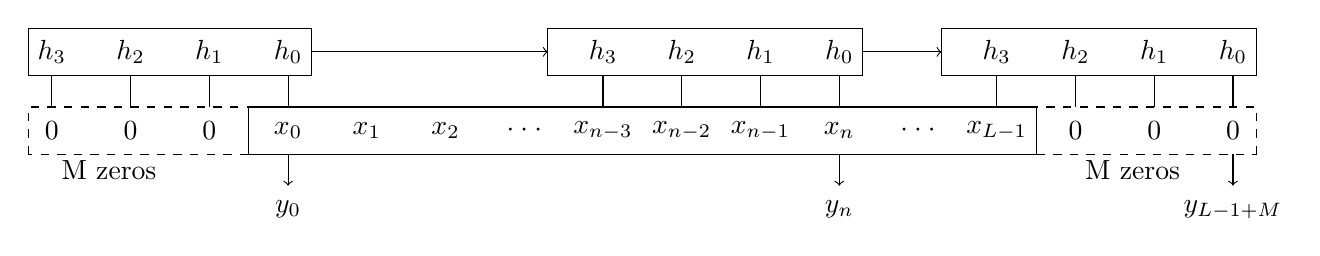
\begin{tikzpicture}

\foreach \h in {0,...,3} {
	\node at (3-\h,0) {$h_{\h}$};
	\node at (10-\h,0) {$h_{\h}$};
	\node at (15-\h,0) {$h_{\h}$};
	
};
\foreach \x in {0,...,2} {
	\node at (3+\x,-1) {$x_{\x}$};
};
\foreach \0 in {0,1,2,13,14,15} {
	\node at (\0,-1) {0};
};

\node at (6,-1) {$\cdot\cdot\cdot$};
\node at (7,-1) {$x_{n-3}$};
\node at (8,-1) {$x_{n-2}$};
\node at (9,-1) {$x_{n-1}$};
\node at (10,-1) {$x_{n}$};
\node at (11,-1) {$\cdot\cdot\cdot$};
\node at (12,-1) {$x_{L-1}$};

\draw (-0.3,0.3) rectangle (3.3,-0.3);
\draw (6.3,0.3) rectangle (10.3,-0.3);
\draw (11.3,0.3) rectangle (15.3,-0.3);
\draw (2.5,-0.7) rectangle (12.5,-1.3);
\draw [dashed] (-0.3,-1.3) rectangle (2.5,-0.7);
\draw [dashed] (15.3,-1.3) rectangle (12.5,-0.7);

\foreach \x in {0,1,2,3,7,8,9,10,12,13,14,15} {
	\draw (\x,-0.3) -- (\x,-0.7);
};

\draw [->] (3.3,0) -- (6.3,0);
\draw [->] (10.3,0) -- (11.3,0);
\foreach \x in {3,10,15} {
	\draw [->] (\x, -1.3) -- (\x,-1.7);
};

\node at (0,-1.5) [anchor=west] {M zeros};
\node at (13,-1.5) [anchor=west] {M zeros};

\node at (3,-2) {$y_0$};
\node at (10,-2) {$y_n$};
\node at (15,-2) {$y_{L-1+M}$};

\end{tikzpicture}
\[
	y(n) = h_0x_n + h_1x_{n-1}+\cdot\cdot\cdot+h_Mx_{n-M}
\]

\subsubsection{Overlap-Add Form\buchSeite{143,144}}
\begin{enumerate}
  \item Divide input $x$ into smaller blocks $x_0, x_1, \ldots$ of length $L$.
  If the input is not long enough for a last complete block, the last block is
  filled up with zeroes
  \item Calculate the output of the convolution of block $x_0$ with $h$,
  resulting in $y_0$
  \item Repeat step 2 for all blocks, resulting in $y_1, y_2, \ldots$
  \item Add $y_0, y_1, \ldots$ up using the following table. $y_{n+1}$ is always
  moved to the right with an offset of $L$ compared to $y_n$.
\end{enumerate}

example: with $L=3$ and $M=3$
\begin{align}
& y_0=h\ast x_0 && y_1=h\ast x_1 && y_2=h\ast x_2 && x={\underbrace{n_0,n_1,n_2},\underbrace{n_3,n_4,n_5},\underbrace{n_6,n_7,n_8}}\notag \\
& && && && \qquad\quad \ x_0 \qquad\quad \ x_1 \qquad\quad \ x_2 \notag
\end{align}\\

\begin{tabular}{c|cccccccccccc}  
	n & 0 & 1 & 2 & 3 & 4 & 5 & 6 & 7 & 8 & 9 & 10 & 11\\
	\hline
	$y_0$ & $y_{0,0}$ & $y_{0,1}$ & $y_{0,2}$ & $y_{0,3}$ & $y_{0,4}$ & $y_{0,5}$ &
	& & & & &\\
	$y_1$ & & & & $y_{1,0}$ & $y_{1,1}$ & $y_{1,2}$ & $y_{1,3}$ & $y_{1,4}$ &
	$y_{1,5}$ & & & \\
	$y_2$ & & & & & & & $y_{2,0}$ & $y_{2,1}$ & $y_{2,2}$ & $y_{2,3}$ & $y_{2,4}$ & $y_{2,5}$
	\\
	\hline
	$y$ & $\Sigma n_{0}$ & $\Sigma n_{1}$&$\Sigma n_{2}$ & $\Sigma n_{3}$&$\Sigma n_{4}$ &$\Sigma n_{5}$ &$\Sigma n_{6}$  &$\Sigma n_{7}$  & $\Sigma n_{8}$ & $\Sigma n_{9}$ & $\Sigma n_{10}$ & $\Sigma n_{11}$
	\\
\end{tabular}


\subsubsection{Transient and Steady-State Behaviour\buchSeite{132,133}}
\begin{multicols}{2}
	\begin{tabular}{|l|l|}
		\hline
		input-on transient	& $ 0 \leq n < M $
		\\ \hline
		steady state			& $ M \leq n \leq L-1 $
		\\ \hline
		input-off transient		& $ L-1 < n \leq L-1+M $
		\\ \hline
	\end{tabular}

\columnbreak

  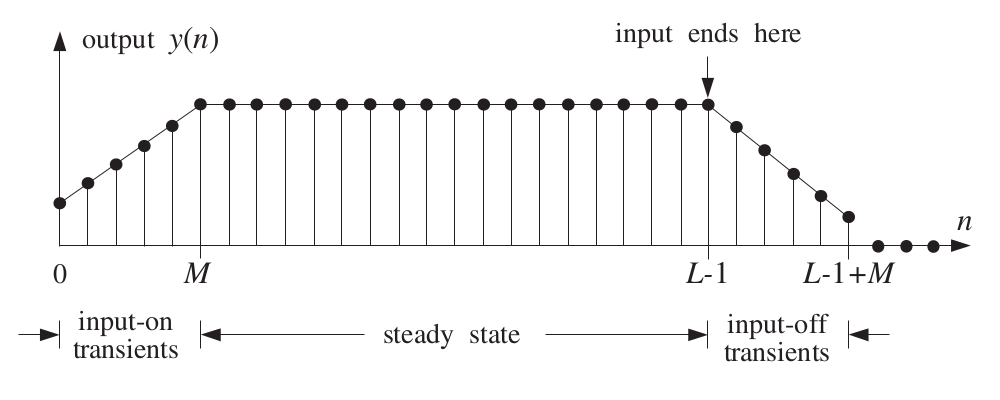
\includegraphics[width=10cm]{./picture/transient_steady_state}
\end{multicols}

Therefore, the direct form takes the following different forms depending
on the value of the output index $n$:
\[
	y_n =
		\left\{
			\begin{array}{l l l}
				\sum\limits_{m=0}^{n} h_m x_{n-m}		& \quad \text{if } 0 \leq n < M			& \quad \text{input-on} \\
				\sum\limits_{m=0}^{M} h_m x_{n-m}		& \quad \text{if } M \leq n \leq L-1	& \quad \text{steady state} \\
				\sum\limits_{m=n-L+1}^{M} h_m x_{n-m}	& \quad \text{if } L-1 < n \leq L-1+M	& \quad \text{input-off}
			\end{array}
		\right.
\]
The DC gain of a stable filter is the steady-state value to which the output converges when the input is a unit step
\[ y_{dc} = \sum_{m}^{} h(m) \qquad y_{dc}=\sum_{m=0}^{\infty}h(m) \]

\subsubsection{Convolution of Infinite Sequences\buchSeite{134}}
Three cases:
\setArrayStretch{1}
\begin{enumerate}
  \item Infinite filter, finite input; i.e., $M = \infty$, $L < \infty$
  \item Finite filter, infinite input; i.e., $M < \infty$, $L = \infty$
  \item Infinite filter, infinite input; i.e., $M = \infty$, $L = \infty$
\end{enumerate}
\resetArrayStretch

Therefore, the direct form takes the following different forms (See also \ref{geometricseries} \nameref{geometricseries}):
\[
	y_n =
		\left\{
			\begin{array}{r l l}
				\sum\limits_{m=max(0,n-L+1)}^{n} & h_m x_{n-m}		& \quad \text{if $M = \infty$, $L < \infty$} \\	
				\sum\limits_{m=0}^{min(n,M)} & h_m x_{n-m}		& \quad \text{if $M < \infty$, $L = \infty$ } \\
				\sum\limits_{m=0}^{n} & h_m x_{n-m}	& \quad \text{if $M = \infty$, $L = \infty$ }
			\end{array}
		\right.
\]


\subsection{Sample Processing Methods\buchSeite{146}}
  \begin{multicols}{2}
    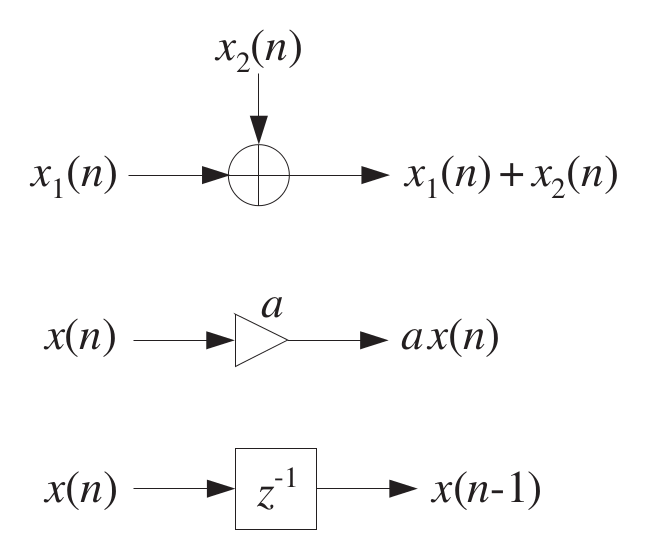
\includegraphics[width=5cm]{./picture/basic_blocks}
    
  \columnbreak
  
    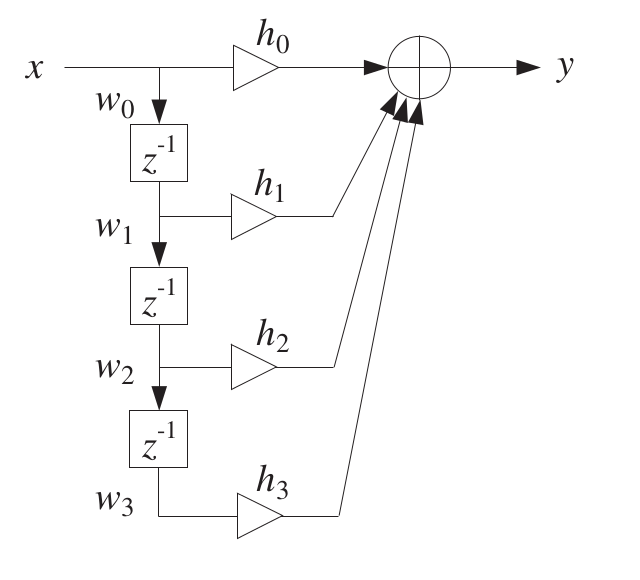
\includegraphics[width=5cm]{./picture/bd_internal_states}
  \end{multicols}
\subsubsection{Pure Delays\buchSeite{147-151}}
\subsubsection{FIR Filtering in Direct Form\buchSeite{152-156}}
\subsubsection{Hardware realizations and circular buffers \buchSeite{162}}